\chapter{Appendix}
\appendix
\newpage
\section{Gantt Chart, part 1}\label{Gantt1}
\begin{figure}[h!]
    \centering
    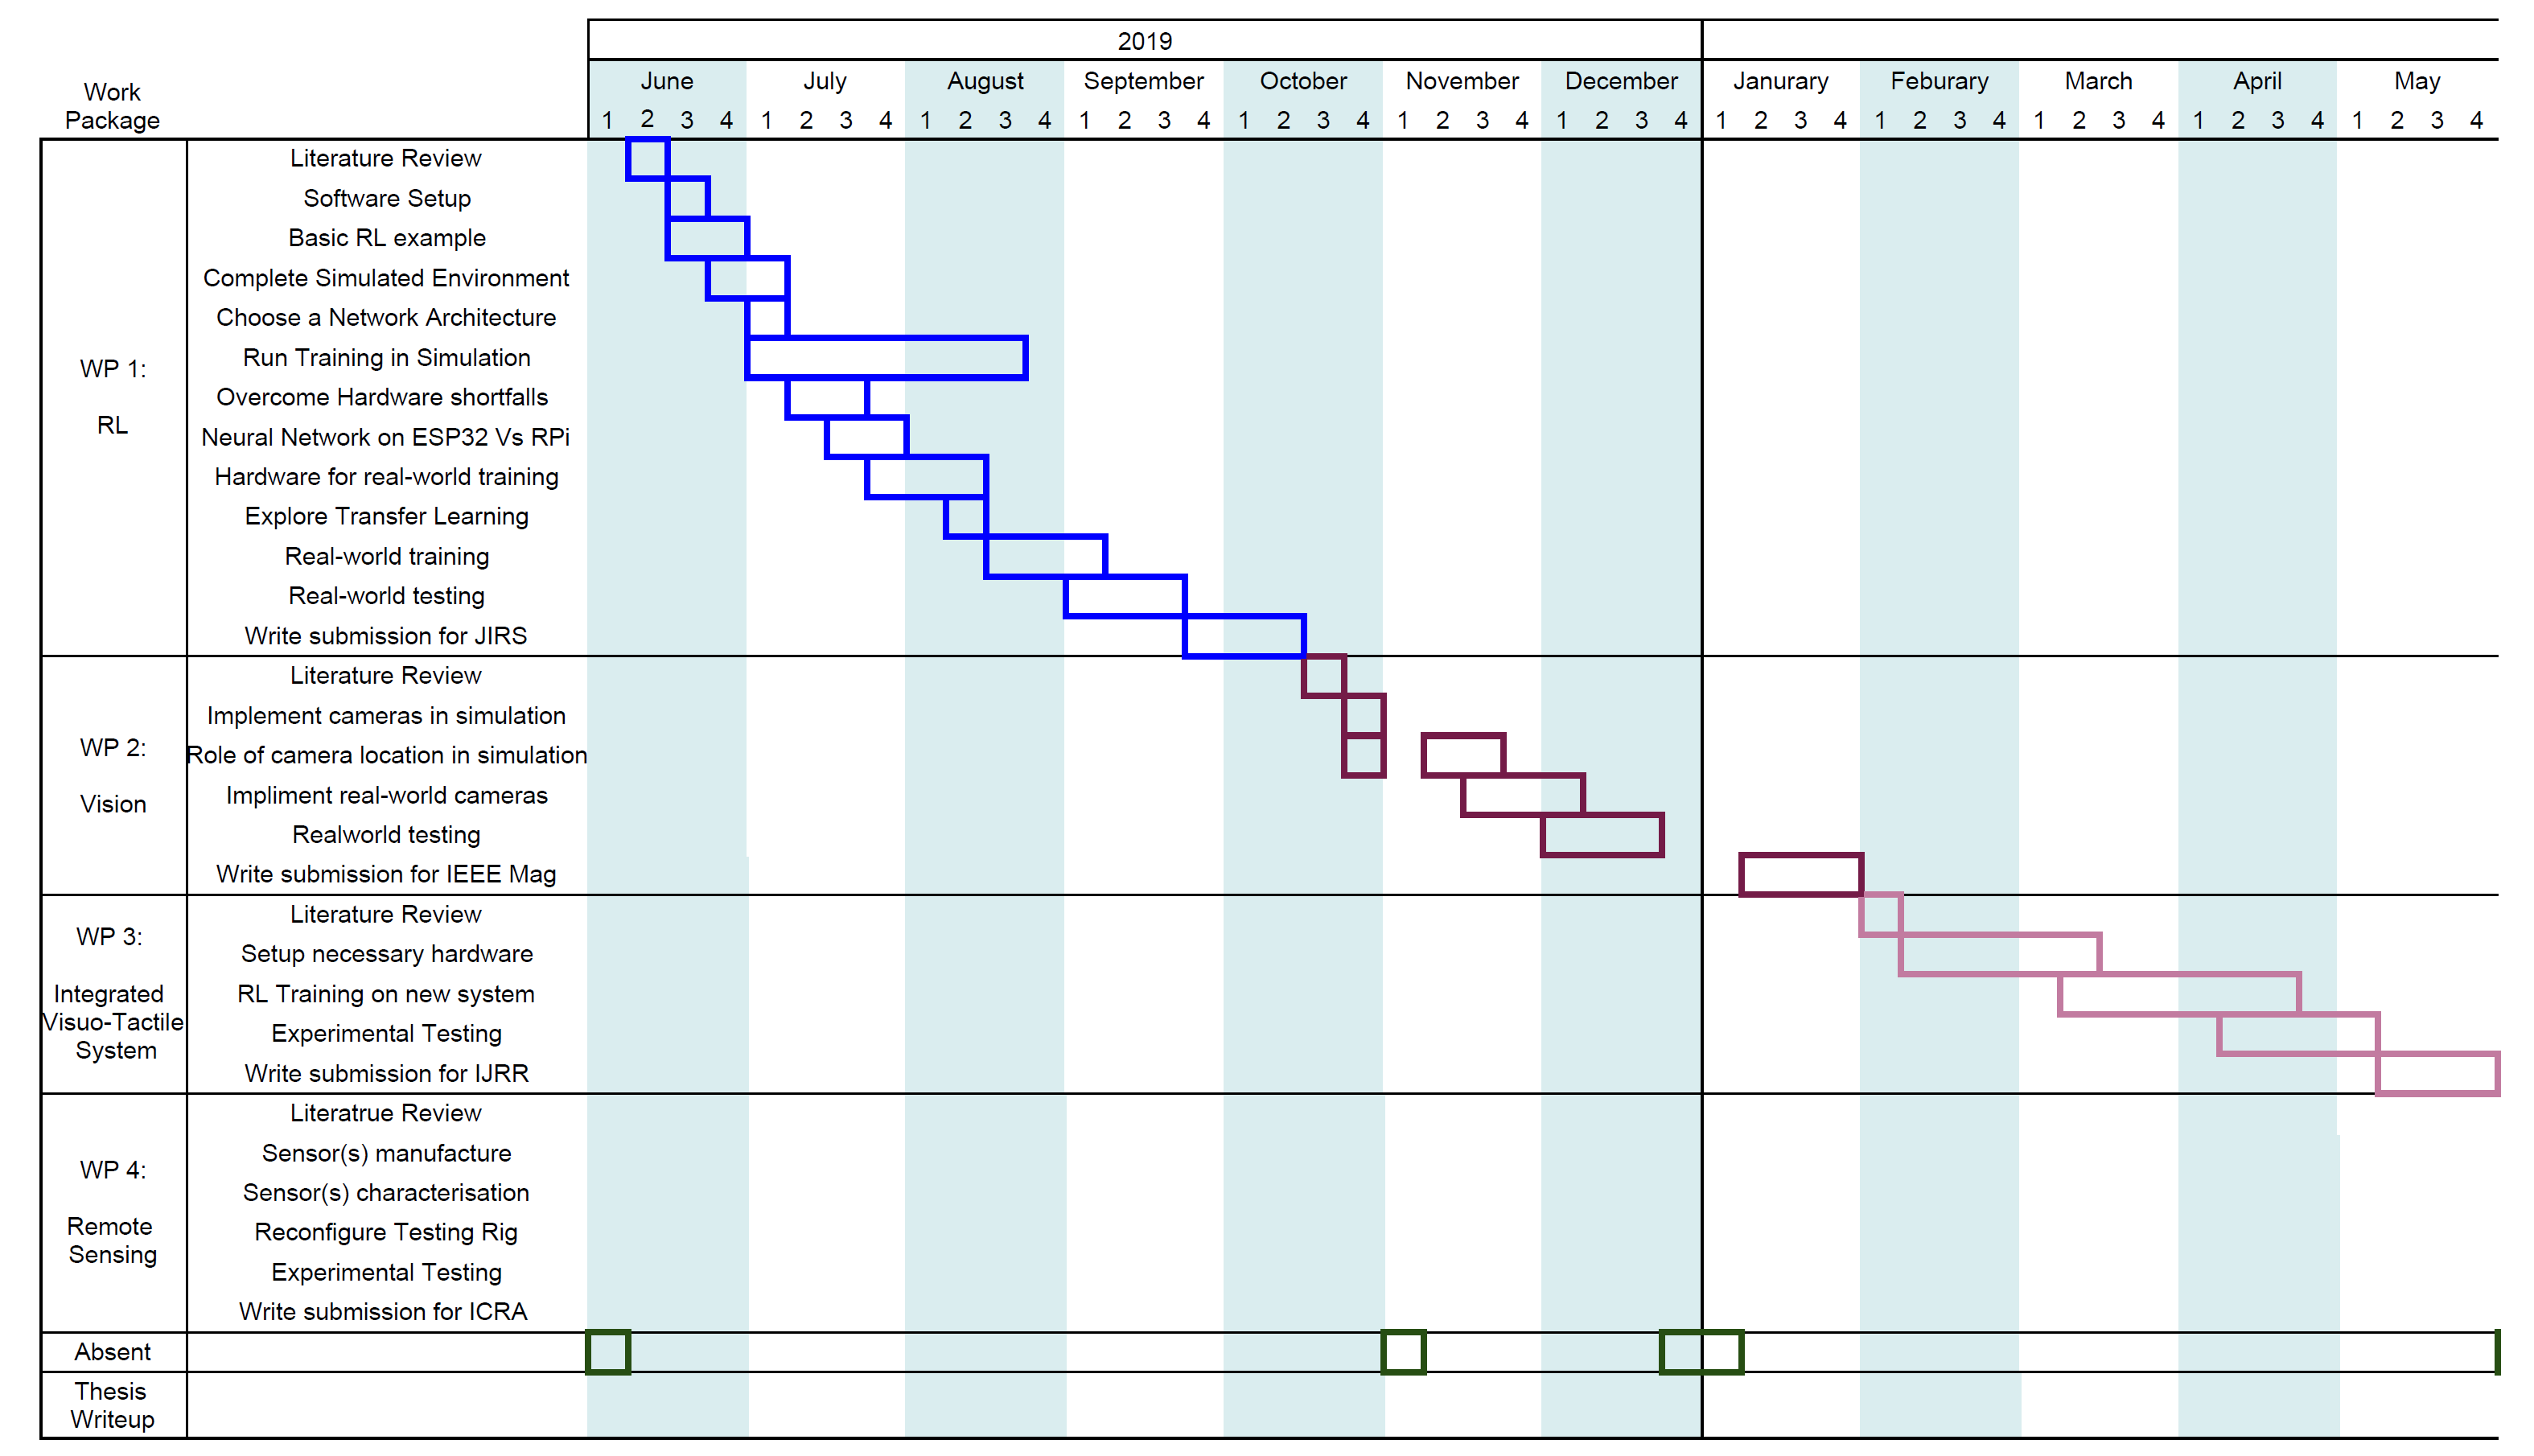
\includegraphics[width=0.93\textheight, angle=270]{Images/GanttChart/Gantt1.png}
%    \caption{Gantt Chart outlining future work, Part 1}
%    \label{Gantt1}
\end{figure}
\newpage
\section{Gantt Chart, part 2}\label{Gantt2}
\begin{figure}[h!]
    \centering
    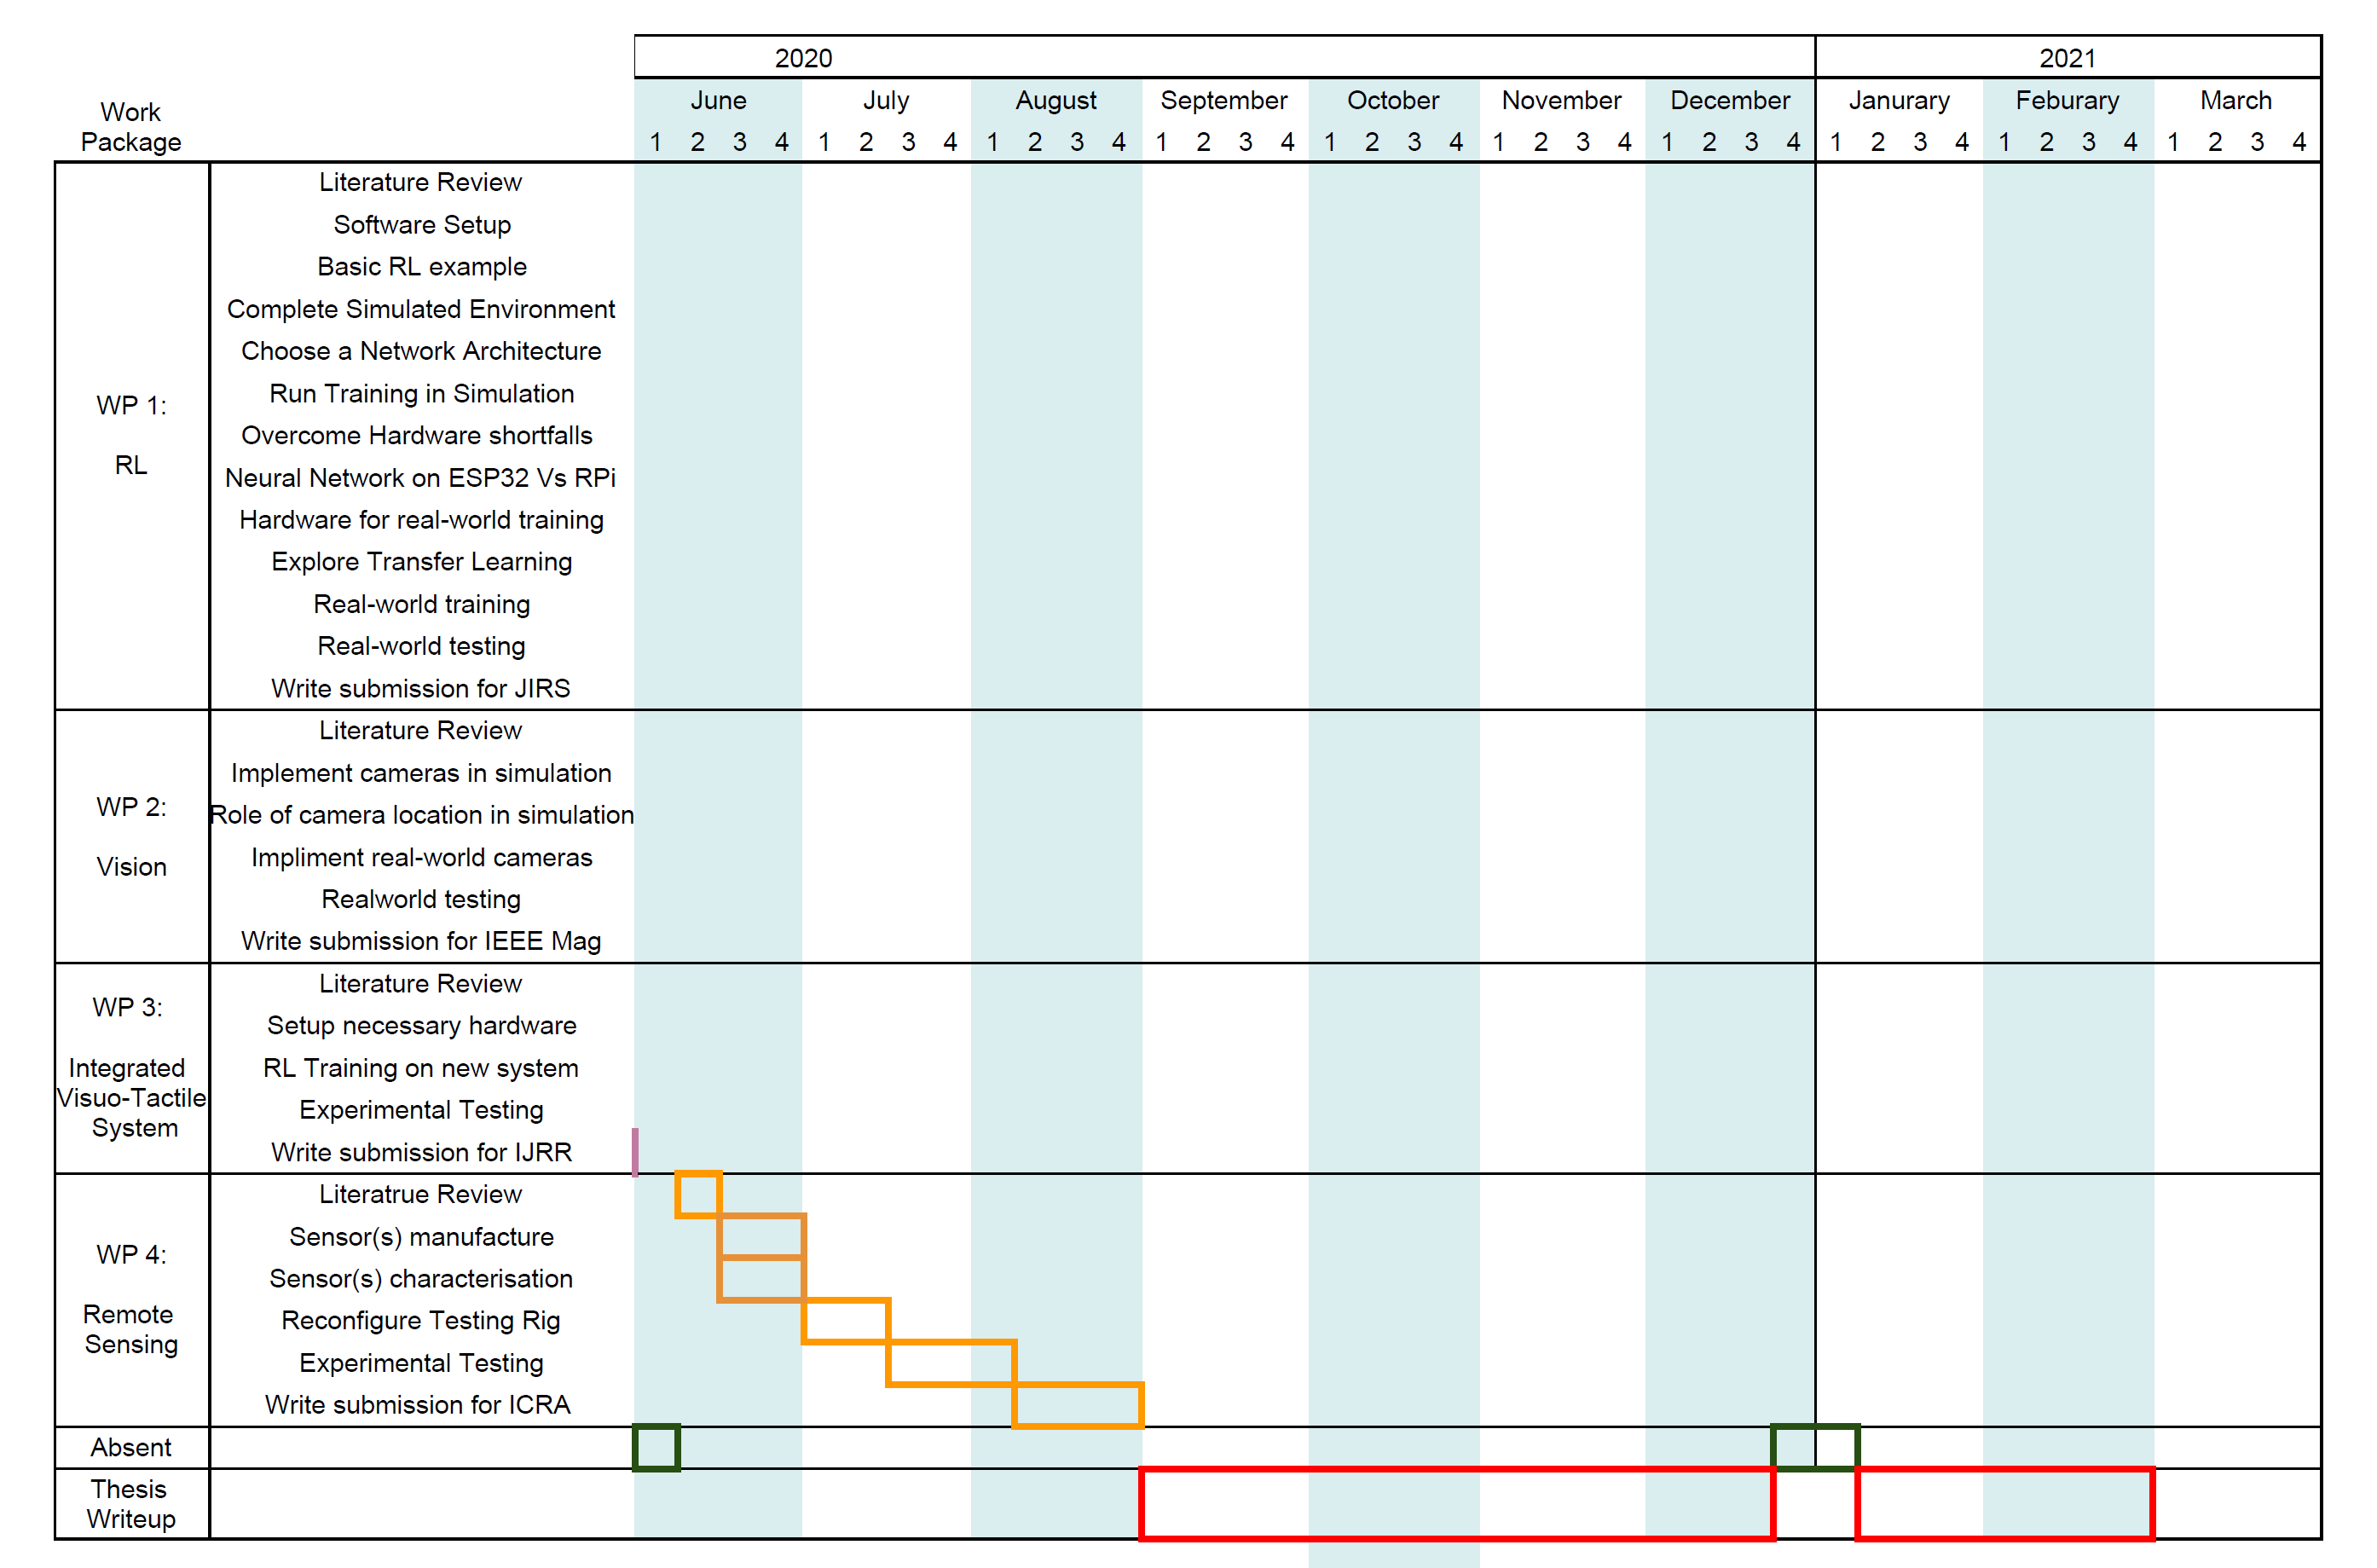
\includegraphics[width=0.93\textheight, angle=270]{Images/GanttChart/Gantt2.png}
%    \caption{Appendix 2: Gantt Chart outlining future work, Part 2}
%    \label{Gantt2}
\end{figure}

\newpage

\section{Gantt Breakdown, Work Package 1}\label{GanttBreakdownWP1}
\begin{itemize}
    \item Literature Review
    
    Read the relevant literature to ensure understanding of the state of the art and check validity of the research question.
    \item Software Setup
    
    Software installation and configuration. Tensorflow, Keras, Gazebo, Blender.
    \item Basic RL example 
    
    Run simple sample program which uses RL, this will be the mountain car problem provided in tensorflow. This will refresh machine learning knowledge and get familiar with the tools and any updates since I last used them.
    \item Complete Simulated Environment 
    
    Complete simulation of the gripper in gazebo. Configure gazebo such that the program can be launch and (unattended) it will run the grasp test iteratively and feed the results into tensorflow for RL. This is essential to achieve the large number of training cycles which is required to make RL feasible.
    \item Choose a Network Architecture
    
    Use existing research and ask people I know in the area to help choose a suitable or a short list of suitable existing neural network architectures for this application.
    \item Run Training in Simulation
    
    Start running training using the simulation. Starting with simulation will allow quick iteration on network architecture, training parameters, etc.
    \item Overcome Hardware shortfalls
    
    Several shortcomings where identified in the experimental rig used for testing for submission in IROS2019. These should be addressed before the same experimental setup is reused.
    \item Neural Network on ESP32 vs RPi
    
    Decide, through experimentation if necessary and documentation if possible, wether to continue development on an ESP32 or a Raspberry Pi
    \item Hardware for real-world training 
    
    The existing gripper will be set up and configured so that it is being controlled by the network in training. This includes the network-rig integration and the sensor integration.
    \item Explore Transfer Learning
    
    Decide if transfer learning is a viable and/or effective option, using experimentation and literature
    \item Real-world training
    
    Taken the lessons learnt from training in simulation into account, training on the real world robotic system will begin. It will take much longer to achieve the same number of training cycles in the real world relative to simulation and therefore some of the complications should be ironed out first in simulation
    \item Write submission for JIRS
    
    JIRS has been identified as a suitable publication to submit to. It is particularly relevant for the research since it focuses on inteligent control, mobile robots, sensors, sensor-fusion and sensor based control.

\newpage

\section{Gantt Breakdown, Work Package 2}\label{GanttBreakdownWP2}
    \item Literature Review
    
    Read the relevant literature to ensure understanding of the state of the art and check validity of the research question.
    \item Implement cameras in simulation
    
    Adapt simulation used in previous work package and implement cameras in different locations. Tip of the finger, wrist, robot torso and robot head. Implement basic computer vision, ball tracking algorithms.
    \item Role of camera location in simulation
    
    Address the core research question through simulation. What is the effect of the location of the camera, accounting for occulusion, resolution, processing speed, latency, implementation concerns, etc.
    \item Implement real world cameras
    
    Integrate ESP32 cam on existing experimental rig.
    \item Real world testing
    
    Verify findings of simulation testing on the experimental rig.
    \item Write Submission for IEEE Mag
    
    IEEE Robotics and Automation Magazine has been identified as a suitable candidate for publication of this research. They have a high impact factor and “focus on working systems and encourage creative solutions to real-world problems and highlighting implementation details”

\newpage

\section{Gantt Breakdown, Work Package 3}\label{GanttBreakdownWP3}
    \item Literature Review
    
    Read the relevant literature to ensure understanding of the state of the art and check the validity of the research question.
    \item Setup necessary hardware
    
    Set up gripper and testing rig with the necessary sensors, etc.
    \item RL Training on new system
    
    Train the new robotic system using Reinforcement learning
    \item Experimental Testing
    
    Benchmark the neural network against a similar network without vision and without tactile. Benchmark against a system using a rule based grasping stragety.
    \item Write Submission for IJRR
    
    IJRR has been identified as a suitable publication for this research as it is currently envisioned. IJRR is the highest ranked robotics journal and this publication would be the culmination of all research in this project to date, combining tactile sensing, reactive grasping, vision sensing and reinforcement learning.
    
    \newpage
    
\section{Gantt Breakdown, Work Package 4}\label{GanttBreakdownWP4}
    \item Literature Review
    
    Read the literature to ensure understanding of the state of the art and check the validity of the research question.
    \item Sensor(s) Manufacture
    
    Develop the sensor(s) which will tested as part of this work package. Light, sonar and wifi are all sensors I would like to test but still need to research the feasibility of each of these.
    \item Sensor(s) characterisation
    
    It is important to properly test the sensor and determine its accuracy, robustness, precision, latency, etc.
    \item Reconfigure Testing Rig
    
    Integrate sensor on gripper and ready the testing rig for testing
    \item Experimental Testing
    
    Conduct real world testing to access the usfullness of a remote tactile sensor to informing the grasping motion for grasping moving objects
    \item Write submissions for ICRA
    
    Identified as a suitable conference with a submission deadline around the correct time of year (~September).

    \newpage

\section{Gantt Breakdown, Misc}\label{GanttBreakdownmisc}
    \item Absent
    
    Foreseeable trips, hoildays, etc.
    \item Thesis Writeup
    
    6 months set aside for writing my final thesis document.

\end{itemize}






